% !TeX root = tcolorbox.tex
% include file of tcolorbox.tex (manual of the LaTeX package tcolorbox)
\clearpage
\section{并排}\label{sec:sidebyside}%
\tcbset{external/prefix=external/sidebyside_}%

\emph{并排}文本框是一种特殊的 \refEnv{tcolorbox}，
其上部分与下部分被左右并排排列。此类文本框均不可断开。

\begin{marker}
  面向代码示例的其他并排选项有
  \refKey{/tcb/listing side text}、
  \refKey{/tcb/text side listing}、
  \refKey{/tcb/listing outside text} 与
  \refKey{/tcb/text outside listing}。
\end{marker}

\subsection{基本设置}\label{subsec:sidebyside_basic}

\begin{docTcbKey}{sidebyside}{\colOpt{=true\textbar false}}{默认 |true|，初始 |false|}
通常，文本框的上部与下部按其名称所示上下排布。
若将 |sidebyside| 设为 |true|，则上部排在\emph{左侧}，下部排在\emph{右侧}。
两部分共用上部的几何设置，但空间按以下选项水平划分。
颜色、字体与框内容追加分别独立使用。
所得文本框不可断开。

\begin{dispExample}
\tcbset{colback=red!5!white,colframe=red!75!black,fonttitle=\bfseries}

\begin{tcolorbox}[title=My title,sidebyside]
  This is the upper (\textit{left-handed}) part.
\tcblower
  This is the lower (\textit{right-handed}) part.
\end{tcolorbox}
\end{dispExample}


\begin{dispExample}
% \usepackage{lipsum}
% \tcbuselibrary{skins}
\begin{tcolorbox}[bicolor,sidebyside,righthand width=3cm,
    sharp corners,boxrule=.4pt,colback=green!5,colbacklower=green!50!black!50]
  \lipsum[2]
\tcblower
  
\includegraphics[width=\linewidth]{goldshade}%
\end{tcolorbox}
\end{dispExample}
\end{docTcbKey}



\clearpage
\begin{docTcbKey}[][doc updated=2024-11-26]{sidebyside align}{=\meta{alignment}}{无默认值，初始 |center|}
  设置左侧与右侧部分的竖直 \meta{对齐方式}。

  \meta{对齐方式}的可选值为：
  \begin{itemize}
  \item\docValue{center}：等同于 |minipage| 选项 |c|。
  \item\docValue{top}：等同于 |minipage| 选项 |t|
    （按基线对齐左右两侧的顶行）。
    \begin{marker}
    自 6.0.0 版本（2023-02-10）起，该 \meta{对齐方式}值需要 \refPkg{luacolor}
    才能正常工作。作为替代，添加 |\strut| 或许有助于模拟等高字体的效果。
    \end{marker}
  \item\docValue{bottom}：等同于 |minipage| 选项 |b|
    （按基线对齐左右两侧的底行）。
  \item\docValue{center seam}：对齐左右两侧的中线。
  \item\docValue{top seam}：对齐左右两侧最顶端的接缝。
  \item\docValue{bottom seam}：对齐左右两侧最底端的接缝。
  \end{itemize}

\begin{exdispExample}{sidebyside_align}
\tcbset{colback=red!5!white,colframe=red!75!black,fonttitle=\bfseries,nobeforeafter,
  left=2mm,right=2mm,sidebyside,sidebyside gap=6mm,width=(\linewidth-2mm)/3}

\begin{tcolorbox}[adjusted title=center,sidebyside align=center]
This is a text which is too long for one line.
\tcblower
This is a short text.
\end{tcolorbox}\hfill
\begin{tcolorbox}[adjusted title=top,sidebyside align=top]
This is a text which is too long for one line.
\tcblower
This is a short text.
\end{tcolorbox}\hfill
\begin{tcolorbox}[adjusted title=bottom,sidebyside align=bottom]
This is a text which is too long for one line.
\tcblower
This is a short text.
\end{tcolorbox}
\end{exdispExample}


\docValue{center}、\docValue{top} 与 \docValue{bottom}
与已知的相应 |minipage| 选项相同。对于文本内容，这是首选方式；
但对于表格或图片等成块内容，结果可能不尽如人意。

对于此类内容，可以使用 \docValue{center seam}、\docValue{top seam}
与 \docValue{bottom seam}。例如，\docValue{top seam} 会对齐左右两侧
最顶端的接缝。


\begin{dispExample}
\tcbset{colback=red!5!white,colframe=red!75!black,fonttitle=\bfseries,
  size=small,righthand width=4cm,sidebyside,sidebyside gap=6mm,lower separated=false}

\begin{tcolorbox}[adjusted title=center seam,sidebyside align=center seam]
  This is my description text for the pictures displayed on the right-handed side.
  \tcblower
  
\includegraphics[width=\linewidth/2]{goldshade}%
  
\includegraphics[width=\linewidth/2]{blueshade}
\end{tcolorbox}

\begin{tcolorbox}[adjusted title=top seam,sidebyside align=top seam]
  This is my description text for the pictures displayed on the right-handed side.
  \tcblower
  
\includegraphics[width=\linewidth/2]{goldshade}%
  
\includegraphics[width=\linewidth/2]{blueshade}
\end{tcolorbox}

\begin{tcolorbox}[adjusted title=bottom seam,sidebyside align=bottom seam]
  This is my description text for the pictures displayed on the right-handed side.
  \tcblower
  
\includegraphics[width=\linewidth/2]{goldshade}%
  
\includegraphics[width=\linewidth/2]{blueshade}
\end{tcolorbox}
\end{dispExample}



\end{docTcbKey}

\clearpage
\begin{docTcbKey}{sidebyside gap}{=\meta{length}}{无默认值，初始 |10mm|}
  将左侧与右侧部分之间的水平间距设为 \meta{长度}。
\begin{dispExample}
\tcbset{colback=red!5!white,colframe=red!75!black,fonttitle=\bfseries,nobeforeafter,
  sidebyside,width=(\linewidth-2mm)/2}

\begin{tcolorbox}[adjusted title=Wide gap,sidebyside gap=30mm]
This is a text which is too long for one line.
\tcblower
This is a short text.
\end{tcolorbox}\hfill
\begin{tcolorbox}[adjusted title=Narrow gap,sidebyside gap=1mm]
This is a text which is too long for one line.
\tcblower
This is a short text.
\end{tcolorbox}
\end{dispExample}
\end{docTcbKey}


\begin{docTcbKey}{lefthand width}{=\meta{length}}{无默认值，初始未设置}
  将左侧部分的宽度设为所给 \meta{长度}。
\begin{dispExample}
\tcbset{colback=red!5!white,colframe=red!75!black,fonttitle=\bfseries}

\begin{tcolorbox}[title=My title,sidebyside,lefthand width=3cm]
This is the upper (\textit{left-handed}) part.
\tcblower
This is the lower (\textit{right-handed}) part.
\end{tcolorbox}
\end{dispExample}
\end{docTcbKey}

\enlargethispage*{1cm}
\begin{docTcbKey}{righthand width}{=\meta{length}}{无默认值，初始未设置}
  将右侧部分的宽度设为所给 \meta{长度}。
\begin{dispExample}
\tcbset{colback=red!5!white,colframe=red!75!black,fonttitle=\bfseries}

\begin{tcolorbox}[title=My title,sidebyside,righthand width=3cm]
This is the upper (\textit{left-handed}) part.
\tcblower
This is the lower (\textit{right-handed}) part.
\end{tcolorbox}
\end{dispExample}
\end{docTcbKey}

\clearpage
\begin{docTcbKey}{lefthand ratio}{=\meta{fraction}}{无默认值，初始 |0.5|}
  将左侧部分的宽度设为可用空间的所给 \meta{比例}。
  \meta{比例}是介于 |0| 与 |1| 之间的值。
\begin{dispExample}
\tcbset{colback=red!5!white,colframe=red!75!black,fonttitle=\bfseries}

\begin{tcolorbox}[title=My title,sidebyside,lefthand ratio=0.25]
This is the upper (\textit{left-handed}) part.
\tcblower
This is the lower (\textit{right-handed}) part.
\end{tcolorbox}
\end{dispExample}
\end{docTcbKey}


\begin{docTcbKey}{righthand ratio}{=\meta{fraction}}{无默认值，初始 |0.5|}
  将右侧部分的宽度设为可用空间的所给 \meta{比例}。
  \meta{比例}是介于 |0| 与 |1| 之间的值。
\begin{dispExample}
\tcbset{colback=red!5!white,colframe=red!75!black,fonttitle=\bfseries}

\begin{tcolorbox}[title=My title,sidebyside,righthand ratio=0.25]
This is the upper (\textit{left-handed}) part.
\tcblower
This is the lower (\textit{right-handed}) part.
\end{tcolorbox}
\end{dispExample}
\end{docTcbKey}


\clearpage
若希望并排文本框的某一侧宽度贴合其内容，必须预先计算出该宽度。
下面的示例使用一个保存盒 |\mysavebox| 来存放图片，以确定其宽度。
处理此任务更便捷的方式是使用 \zvref{subsec:sidebyside_xparse} 中的方法。

\begin{dispExample}
% \tcbuselibrary{skins}
% \usepackage{lipsum}
% \newsavebox\mysavebox  % preamble
\DeclareTotalTColorBox \mysidebox { O{} +m +m }{
  bicolor,colback=white,colbacklower=yellow!10,
  fonttitle=\bfseries,center title,
  sidebyside,
  code={\sbox{\mysavebox}{#2}},
  lefthand width=\wd\mysavebox,
  drop lifted shadow,
  #1
}
{\usebox{\mysavebox}\tcblower#3}

\mysidebox[title=The Triangle]{%
  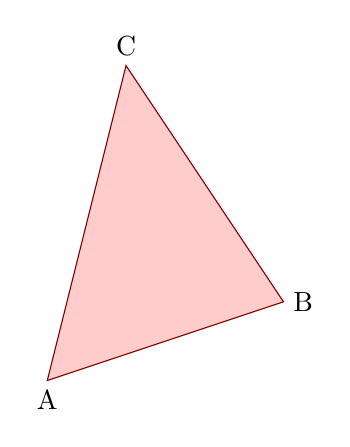
\begin{tikzpicture}
    \path[fill=red!20,draw=red!50!black]
      (0,0) node[below]{A} -- (3,1) node[right]{B}
      -- (1,4) node[above]{C} -- cycle;
  \end{tikzpicture}%
}{%
  \lipsum[1]
}
\end{dispExample}


\clearpage
\subsection{高级设置}\label{subsec:sidebyside_xparse}


\begin{docCommand}[doc new=2015-11-20]{tcbsidebyside}{\oarg{options}\marg{left-handed content}\marg{right-handed content}}
  使用任意（或多或少的）\meta{选项}为 \refEnv{tcolorbox} 创建一个彩色文本框。
  \refKey{/tcb/sidebyside} 选项被设为 |true|，
  并把 \meta{左侧内容}与 \meta{右侧内容}相应地填入文本框。
  所得文本框不可断开。

  \refCom{tcbsidebyside} 不仅是“使用带 \refKey{/tcb/sidebyside} 的普通
  \refEnv{tcolorbox}”的快捷方式，还允许设置
  \refKey{/tcb/sidebyside adapt} 与 \refKey{/tcb/sidebyside switch} 等进一步选项。


\begin{dispExample}
% \tcbuselibrary{skins}
% \usepackage{lipsum}
\tcbsidebyside[title=The Triangle,
  sidebyside adapt=left,
  bicolor,colback=white,colbacklower=yellow!10,
  fonttitle=\bfseries,center title,drop lifted shadow,
]{%
  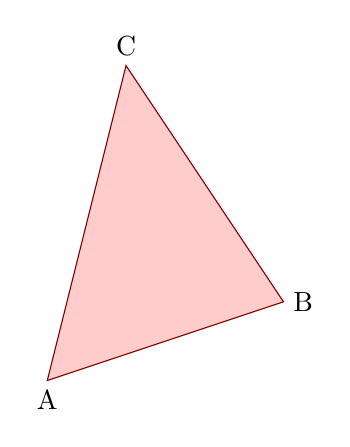
\begin{tikzpicture}
    \path[fill=red!20,draw=red!50!black]
      (0,0) node[below]{A} -- (3,1) node[right]{B}
      -- (1,4) node[above]{C} -- cycle;
  \end{tikzpicture}%
}{%
  \lipsum[1]
}
\end{dispExample}
\end{docCommand}


\clearpage
\begin{docTcbKey}[][doc new=2015-11-20]{sidebyside adapt}{=\meta{side(s)}}{无默认值，初始 |none|}
  本选项允许由左侧和/或右侧来决定文本框的尺寸。
  本选项仅在 \refCom{tcbsidebyside} 内部有效。

\meta{侧}的可选值为：
\begin{itemize}
\item\docValue{none}：不测量左右两侧。
\item\docValue{left}：
  用左侧内容的实际宽度设置 \refKey{/tcb/lefthand width}。
\item\docValue{right}：
  用右侧内容的实际宽度设置 \refKey{/tcb/righthand width}。
\item\docValue{both}：
  用左右两侧内容的实际宽度设置
  \refKey{/tcb/lefthand width}、\refKey{/tcb/righthand width}
  以及整体的 \refKey{/tcb/width}。
\end{itemize}

\begin{dispExample}
% \tcbuselibrary{skins}
\tcbsidebyside[sidebyside adapt=left,
  title=Very important table,
  beamer,colframe=blue!50!black,colback=blue!10,
  lower separated=false,sidebyside gap=5mm
]{%
  \begin{tabular}{|l|c|r|}\hline
    left & center & right\\\hline
    A & B & C\\\hline
    D & E & F\\\hline
  \end{tabular}
}{%
  This table contains the most important figures for
  all future actions. You may notice that B follows A,
  C follows B, and so on.
}
\end{dispExample}



\begin{dispExample}
% \tcbuselibrary{skins}
\tcbsidebyside[sidebyside adapt=right,
  blanker,sidebyside gap=5mm
]{%
  \lipsum[2]
}{%

\begin{tikzpicture}
  \path[fill=yellow,draw=yellow!75!red] (0,0) circle (1cm);
  \fill[red] (45:5mm) circle (1mm);
  \fill[red] (135:5mm) circle (1mm);
  \draw[line width=1mm,red] (215:5mm) arc (215:325:5mm);
\end{tikzpicture}
}
\end{dispExample}


\begin{dispExample}
% \tcbuselibrary{skins}
\tcbsidebyside[sidebyside adapt=both,
  enhanced,center,
  title=Both sides adapted,
  attach boxed title to top center={yshift=-2mm},
  coltitle=black,boxed title style={colback=red!25},
  segmentation style=solid,colback=red!5,colframe=red!50
]{%
  \begin{tabular}{|l|c|r|}\hline
    left & center & right\\\hline
    A & B & C\\\hline
    D & E & F\\\hline
  \end{tabular}
}{%

\begin{tikzpicture}
  \path[fill=yellow,draw=yellow!75!red] (0,0) circle (1cm);
  \fill[red] (45:5mm) circle (1mm);
  \fill[red] (135:5mm) circle (1mm);
  \draw[line width=1mm,red] (215:5mm) arc (215:325:5mm);
\end{tikzpicture}
}
\end{dispExample}

\end{docTcbKey}


\clearpage
\begin{docTcbKey}[][doc new=2015-11-20]{sidebyside switch}{\colOpt{=true\textbar false}}{默认 |true|，初始 |false|}
  若设为 |true|，则交换 \refCom{tcbsidebyside} 的
  \meta{左侧内容}与 \meta{右侧内容}。
  显然，本选项仅在 \refCom{tcbsidebyside} 内部有效。

  若在 \refKey{/tcb/if odd page} 内部使用，
  还可使左右侧的交换随奇偶页而变化。

\begin{dispExample}
% \tcbuselibrary{skins}
\tcbsidebyside{Left}{Right}

\tcbsidebyside[sidebyside switch]{Left}{Right}

\tcbsidebyside[title=Very important table,
  if odd page={sidebyside switch,sidebyside adapt=right,flushright title}%
              {sidebyside adapt=left},
  beamer,colframe=blue!50!black,colback=blue!10,
  lower separated=false,sidebyside gap=5mm
]{%
  \begin{tabular}{|l|c|r|}\hline
    left & center & right\\\hline
    A & B & C\\\hline
    D & E & F\\\hline
  \end{tabular}
}{%
  This table contains the most important figures for
  all future actions. You may notice that B follows A,
  C follows B, and so on.
}
\end{dispExample}


\end{docTcbKey}

